With a density of 1.27 \unit{\gram\per\cubic\centi\meter} according to the \textit{ESTAR Database} \cite{ESTAR}, the plastic shows a clear build-up effect that becomes more notable as the energy of the incoming beam rises. Using the \textbf{plane neutron source}, the tissue equivalent cylinder behaves as follows:

\begin{figure}[!h]
\centering
\begin{minipage}[t]{0.8\textwidth}
    \centering
    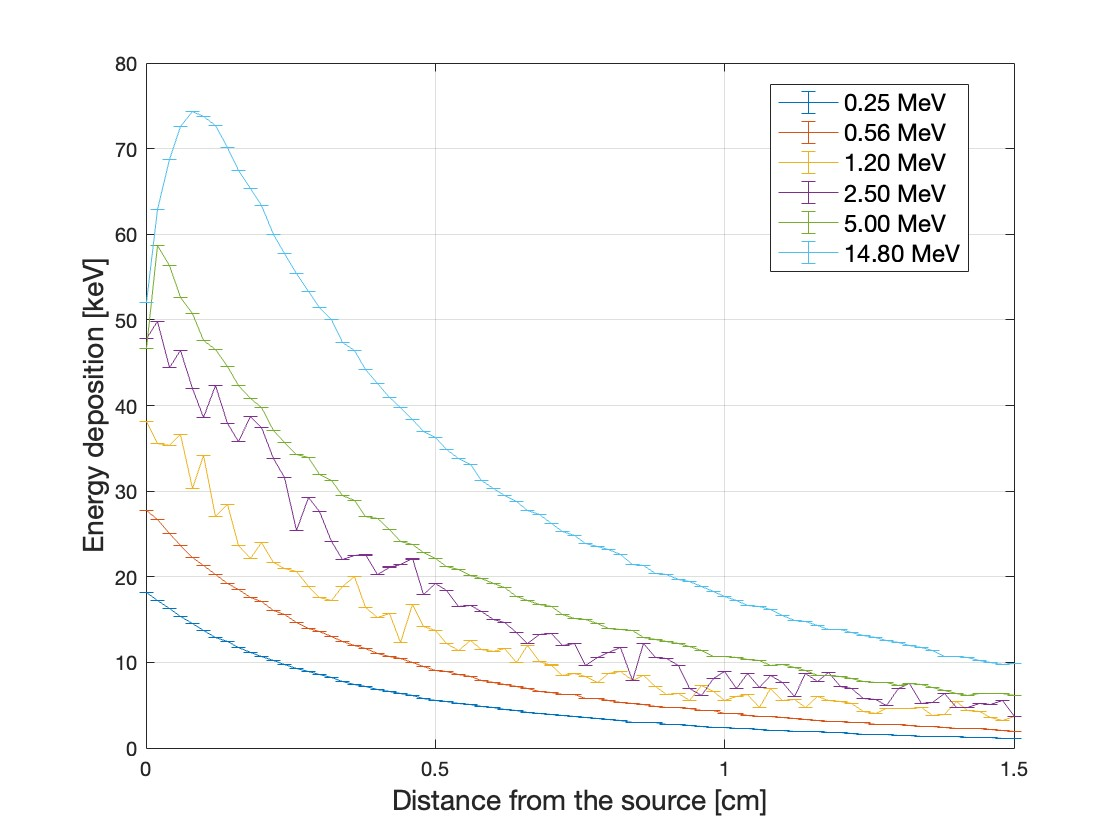
\includegraphics[width=\linewidth, height=9cm]{Master Thesis Manuel Galdon/figures/Build-up effect/TE cylinder with plane source.jpg} 
    \caption{Energy deposition plot of a TE cylinder plot using a plane neutron source at different energies. There is no gap between the source plane and the cylinder.}
    \label{fig:A150 cylinder with plane neutron source}
\end{minipage}
\end{figure}

Here, neutrons are primarily scattered by the constituent nuclei. As these neutrons travel deeper into the material, they engage in numerous interactions, transferring energy to atomic nuclei and generating secondary charged particles. This chain of interactions results in an increased dose deposition within the plastic at greater depths, which explains the slight displacement of the peak of energy deposition to the right as the energy of the beam increases, giving rise to the buildup effect that is observed beyond the energy of 2.5 \unit{\mega\electronvolt}.
